\lab{Спектральный анализ электрических сигналов}
\aim{изучить спектральный состав периодических электрических сигналов.}

\equip{анализатор спектра (аналоговый или цифровой),
    генератор прямоугольных импульсов и сигналов специальной формы, осциллограф.}

Перед выполнением работы необходимо ознакомиться с теоретическим введением
к разделу.

В~работе изучается спектральный состав периодических электрических сигналов
различной формы: последовательности прямоугольных импульсов, последовательности
цугов и амплитудно-модулированных гармонических колебаний. Спектры этих сигналов
наблюдаются с помощью анализатора спектра и сравниваются c рассчитанными
теоретически.

Периодическая функция может быть представлена в виде бесконечного ряда
гармонических функций --- ряда Фурье (см. п.~\ref{sec:spectrum-periodic}
Введения):
\begin{equation*}
f(t) = \sum_{n=-\infty}^{\infty} c_n e^{in\omega_0 t}\qquad\text{или}\qquad
f=\sum_{n=0}^{\infty} a_n \cos (n\omega_0 t + \varphi_n).
\end{equation*}
Здесь $\omega_0 = 2\pi/T$, где $T$ --- период функции $f(t)$.
Коэффициенты $\{c_n\}$ могут быть найдены по формуле
\chaptereqref{fourier-coeff}:
\begin{equation*}
    c_n=\frac{1}{T}\int\limits_{0}^{T} f(t)e^{-in\omega_0 t}\,dt.
\end{equation*}
\begin{wrapfigure}{o}{0.3\textwidth}
    \centering
    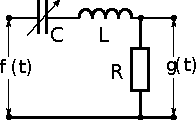
\includegraphics{Chapter_6/6-1-RLC.pdf}
    \caption{Колебательный контур как узкополосный фильтр}
    \figmark{simple-RLC}
\end{wrapfigure}
Наборы коэффициентов разложения в комплексной $\{c_n\}$ и действительной
$\{a_n,\varphi_n\}$ формах связаны соотношением \chaptereqref{Fourier-coefficient}:
\begin{equation*}
a_n = 2|c_n|,\qquad \varphi_n = \arg c_n.
\end{equation*}

В~качестве простейшего спектрального анализатора можно использовать
высокодобротный колебательный контур с подстраиваемой ёмкостью или
индуктивностью, рис.~\figref{simple-RLC}
(см. также п.~\ref{sec:spectrum-meaning} Введения).
Такой контур усиливает те гармоники входного сигнала $f(t)$,
частота которых близка к резонансной
$\nu_{0} = 1/(2\pi\sqrt{LC})$, и практически не реагирует на частоты,
далёкие от~$\nu_{0}$. С~точки зрения преобразования гармоник колебательный контур
является узкополосным \term{фильтром} с шириной полосы
пропускания порядка $\Delta \nu \sim \nu_{0}/ Q$, где $Q =
\frac{1}{R}\sqrt{\frac{L}{C}} \gg 1$~--- его добротность. Амплитуда колебаний
в контуре пропорциональна амплитуде~$|c(\nu_0)|$ гармоники в фурье-спектре функции $f(t)$,
частота которой совпадает с $\nu_{0}$. 
Таким образом, меняя резонансную частоту контура,
можно <<просканировать>> весь спектр входного сигнала.

\experiment

У~описанной выше схемы есть существенный недостаток: при изменении~$L$ или~$C$
меняется также и добротность, а значит и ширина полосы пропускания.
Кроме того, проще изготовить высокодобротный контур с фиксированными параметрами,
нежели с настраиваемой частотой. В~связи с этим, как правило, для фильтрации сигнала
применяется другая схема.

Исследуемый сигнал $f(t)$ и синусоидальный сигнал от вспомогательного генератора,
называемого в таких \term{гетеродином}, подаются на вход \term{смесителя}. 
Смеситель~--- элемент, преобразующий колебания с частотами~$\nu_1$
и~$\nu_2$ в колебания на \important{комбинированных}
частотах: $\nu_1 + \nu_2$ и $\nu_1 - \nu_2$.
<<Разностный>> сигнал смесителя поступает на фильтр ---
высокодобротный колебательный контур, настроенный на некоторую 
\important{фиксированную}
резонансную частоту~$\nu_0$. Таким образом, если $f(t)$ содержит гармонику
$\nu=\nu_{гет}-\nu_0$ ($\nu_{гет}$ --- частота гетеродина), 
она будет усилена, а отклик будет пропорционален её амплитуде.

Отметим, что смешение частот исследуемого сигнала и частоты гетеродина лежит в
основе большинства современных радиоприёмных устройств~---
\important{супергетеродинов}.

\begin{figure}[h!]
\centering
\pic{0.9\textwidth}{Chapter_6/6_1_1}
\caption{Структурная схема анализатора спектра}
\figmark{Spectrum analyzer}
\end{figure}

В~спектральном анализаторе частота гетеродина пропорциональна напряжению,
подаваемому на развертку по оси~$X$ встроенного в анализатор осциллографа.
Выходной сигнал подаётся на канал~$Y$. На экране анализатора возникает, таким
образом, график, изображающий зависимость амплитуды гармоник исходного сигнала
от частоты, т.\,е. его спектр (заметим, что информация о фазах гармоник при этом
теряется).

В~последнее время повсеместное распространение получила цифровая обработка
сигналов. Спектральный состав оцифрованного сигнала может быть найден численно.
Существуют алгоритмы (быстрое преобразование Фурье, FFT), позволяющие проводить
вычисления коэффициентов Фурье в реальном времени для сигналов относительно
высокой частоты (до 200~МГц). Гетеродинные схемы по-прежнему
применяются для анализа спектров сверхвысоких частот, приближающихся
к тактовой частоте современных интегральных схем ($\gtrsim1$~ГГц).

\begin{lab:task}

\taskpreamble{~}
\vspace*{-8ex} % workaround

\tasksection{А. Исследование спектра периодической последовательности прямоугольных
импульсов}

\taskpreamble{В~этом упражнении исследуется зависимость ширины спектра $\Delta \nu$
периодической последовательности прямоугольных импульсов
от длительности отдельного импульса $\tau$.}

\item Ознакомьтесь с устройством приборов (генератор прямоугольных импульсов,
осциллограф, анализатор спектра) и подготовьте их к работе,
следуя техническим описаниям, расположенным на установке.

\begin{figure}[h!]
    \hfil\hfil
    \begin{minipage}{0.45\textwidth}
        \pic{\linewidth}{Chapter_6/6_2_1}
        \caption{Периодическая последовательность импульсов}
    \end{minipage}
    \hfil
    \begin{minipage}{0.45\textwidth}
        \pic{\linewidth}{Chapter_6/6_2_2}
        \caption{Спектр последовательности импульсов 
            (расчёт для $\tau=T/7$)}
    \end{minipage}
\end{figure}

\item Подключите генератор прямоугольных импульсов через разветвитель
к осциллографу и анализатору спектра.

\item На генераторе задайте частоту повторения импульсов
$\nu_{повт} = 1\;кГц$ (период $T=1\;мс$), длительность импульса
$\tau=50\;мкс$. Получите устойчивую картину сигнала на осциллографе.

\item Предварительно оцените характерную ширину спектра
из соотношения неопределённостей $\Delta \nu \sim 1/\tau$
(см.  п.~\ref{sec:indeterminacy} Введения).

\item Получите спектр сигнала на анализаторе спектра. Предварительно
подберите начало отсчёта и диапазон измерения по частоте,
так чтобы на экране помещалась б\'{о}льшая часть спектра.

В~наблюдаемом спектре отсутствует информация об амплитуде нулевой гармоники,
т.е. о~величине постоянной составляющей; её местоположение (начало отсчёта шкалы
частот) отмечено небольшим вертикальным выбросом.

\item\label{item:foto} Измеяя параметры сигнала ($\nu_{повт}$, $\tau$),
наблюдайте, как изменяется его спектр. Опишите результаты.
Сохраните или сфотографируйте несколько огибающих спектров с различными
параметрами, например:
а)~$\nu_{повт}=1\;кГц$, $\tau=50\;мкс$,
б)~$\nu_{повт}=1\;кГц$, $\tau=100\;мкс$,
в)~$\nu_{повт}=2\;кГц$, $\tau=50\;мкс$.
при фиксированном масштабе частот (по оси $X$) анализатора спектра [кГц/дел],
Параметры запишите в тетради, изображения спектров приложите к отчёту.

\item Проведите измерения зависимости ширины спектра от длительности
импульса~$\Delta \nu(\tau)$ при изменении $\tau$ от 25 до 200~мкс при
$\nu_\text{повт}=1$~кГц. Ширину определяйте по положению первой гармоники
с нулевой амплитудой.

\item Постройте график зависимости ширины спектра от обратного времени импусльа
$\Delta \nu(1/\tau)$ и по его наклону убедитесь в справедливости соотношения
неопределённостей. Оцените погрешность данного опыта.

\item Для одного из сигналов, наблюдаемых в п.~\ref{item:foto}, рассчитайте теоретические
значения амплитуд спектральных компонент по формуле \chaptereqref{impulses-spectrum}.
Сравните измеренные значения с теоретическими, изобразив их на одном графике.

\tasksection{Б. Исследование спектра периодической~последовательности цугов
гармонических~колебаний}

\taskpreamble{В~этом упражнении исследуется зависимость расстояния между ближайшими
спектральными компонентами от частоты повторения цугов.}

\begin{figure}[h!]
\hfil\hfil
\begin{minipage}[b]{0.45\textwidth}
     \pic{\linewidth}{Chapter_6/v6-zug-nu}
    \caption{Периодическая последовательность цугов}
\end{minipage}
\hfil
\begin{minipage}[b]{0.45\textwidth}
\centering
     \pic{\linewidth}{Chapter_6/6_1_zugs}
    \caption{Спектр последовательности цугов}
\end{minipage}
\end{figure}


\item По техническому описанию к работе соберите схему, используемую
для генерации последовательности синусоидальных цугов.

\item Установите частоту несущей $\nu_0=25$~кГц и получите на экране осциллографа
устойчивую картину цугов.

\item Получите спектр сигнала. Наблюдайте, как изменяется вид спектра:
а)~при увеличении длительности импульса (например, $\tau=50$, $100$~мкс
для $\nu_\text{повт}=1\;кГц$); б)~при изменении частоты несущей:
$\nu_0=25$,~10 или~40~кГц; в)~при изменении частоты повторения
$\nu_{повт}=1,\;2$~кГц. Опишите результаты или зарисуйте качественную
картину в~тетради.

\item При фиксированной длительности импульсов $\tau=50$~мкс исследуйте
зависимость расстояния~$\delta \nu$ между соседними спектральными компонентами
периода повторения импульсов $T=1/\nu_\text{повт}$
(в~диапазоне частот 1--8~кГц).

\item Постройте график $\delta \nu(1/T)$ и по его наклону
убедитесь в~справедливости соотношения неопределённости.
Оцените погрешность данного опыта.

% \item Сравните зарисованные на кальку спектры:
% \begin{itemize}
% 	\item прямоугольных импульсов при одинаковых периодах и разных
% длительностях импульса $\tau$;
% 	\item цугов при одинаковых $\tau$ и разных периодах;
% 	\item цугов и прямоугольных импульсов при одинаковых значениях~$\tau$
% и~$T$.
% \end{itemize}

\tasksection{В. Исследование спектра гармонических сигналов, модулированных по
амплитуде}

\taskpreamble{В~этом упражнении исследуется зависимость отношения амплитуд спектральных линий
синусоидального сигнала, модулированного низкочастотными гармоническими
колебаниями, от коэффициента модуляции, измеряемого с~помощью осциллографа.}

\begin{figure}[h!]
    \centering
\pic{0.6\textwidth}{Chapter_6/6_1_mod}
    \caption{Модулированный по амплитуде сигнал}
\end{figure}

\item Следуя техническому описанию на установке соберите схему для
генерации гармонических модулированных колебаний.

\item Установите частоту несущей $\nu_0=25\;кГц$, частоту модуляции
$\nu_{мод} = 1\;кГц$ и глубину модуляции $m=1$.
Получите на экране осциллографа устойчивую картину.

\item Получите спектр исследуемого сигнала. Измерьте положения центральной
и боковой гармоник. Изменяя частоту модулирующего сигнала $\nu_{мод}$
и частоту несущей $\nu_0$, наблюдайте, как измеяется положение спектральных линий.
Опишите или зарисуйте результат в тетрадь.

\item Меняя глубину модуляции~$m$, измеряйте отношение $\frac{a_\text{бок}}{a_\text{осн}}$ 
амплитуд боковой и основной линий (см. рис.~\chapterfigref{spectrum-modulated}) 
спектра  в зависимости от~$m$;
для расчёта глубины модуляции~$m$ используйте формулу \chaptereqref{modul-deep}:
\begin{equation*}
    m = \frac{A_{\rm max} - A_{\rm min}}{A_{\rm max} + A_{\rm min}},
\end{equation*}
где максимальная~$A_{\rm max}$ и минимальная~$A_{\rm min}$ амплитуды сигнала
измеряются с помощью осциллографа.

\item Постройте график отношения $a_\text{бок}/a_\text{осн}$
в~зависимости от~$m$. Определите угол наклона графика и сравните
с результатами п.~\ref{sec:modulated-spectrum}. Оцените погрешность данного опыта.

\end{lab:task}



%\lit

%\n \textit{Сивухин Д.В.} Общий курс физики. Т.~III. Электричество~--- М.: Наука,
% 1983. \S~128.

%\n \textit{Крауфорд Ф.} Берклеевский курс физики. Т.~III. Волны.~--- М.: Наука,
% 1976. \S~6.4.
